\chapter{گام ۲: خوشه بندی و انتخاب توالی نماینده}
    پس از شناسایی توالی‌های بالقوه زایلاناز در مرحله 1، به مرحله 2 می‌رویم، که شامل خوشه‌بندی توالی‌های بسیار مشابه برای کاهش افزونگی و انتخاب توالی‌های نماینده از هر خوشه است. این فرآیند تضمین می‌کند که تجزیه و تحلیل‌های بعدی از نظر محاسباتی کارآمد هستند و به جای چندین نسخه اضافی از یک ژن، روی توالی‌های عملکردی متنوع متمرکز هستند.

    خوشه بندی برای مطالعات متاژنومی ضروری است زیرا متاژنوم ها اغلب دارای گونه های ژنی بسیار مشابه هستند. با اعمال الگوریتم های خوشه بندی مانند CD-HIT، می توانیم:
    \begin{itemize}
        \item کاهش بار محاسباتی برای تجزیه و تحلیل پایین دست.
        \item اطمینان حاصل کردن از این که هیچ گونه خاص زایلاناز را بیش از حد نشان نمی دهیم.
        \item با تمرکز بر انواع توالی متمایز، پیش بینی های عملکردی را بهبود میبخشیم.
    \end{itemize}

    در این مرحله، از CD-HIT، یک ابزار خوشه‌بندی پرکاربرد، برای گروه‌بندی توالی‌ها بر اساس آستانه شباهت استفاده می‌کنیم. توالی های نماینده به دست آمده به عنوان یک مجموعه داده غیر زائد برای تجزیه و تحلیل ساختاری و عملکردی بیشتر عمل می کنند.

    \section*{ابزار مورد استفاده: CD-HIT برای خوشه بندی بر اساس آستانه تشابه }
        CD-HIT یک الگوریتم خوشه بندی پرکاربرد برای کاهش افزونگی در مجموعه داده های توالی بزرگ است. توالی‌هایی را گروه‌بندی می‌کند که درصد مشخصی از شباهت را به اشتراک می‌گذارند، و تنها یک دنباله نماینده برای هر خوشه حفظ می‌کند.
        برای این پروژه، CD-HIT به صورت زیر پیکربندی شد:
        \begin{itemize}
            \item آستانه تشابه 
            (0.97): توالی هایی با شباهت 97 درصد یا بیشتر در یک خوشه گروه بندی شدند.
            \item اندازه کلمه (5): اندازه کلمه 5 برای خوشه بندی پروتئین، تعادل سرعت و دقت استفاده شد.
            \item توضیحات (0): فقط اطلاعات توالی ضروری را در خروجی حفظ می کند.
        \end{itemize}
        \section{دستورات ترمینال برای خوشه بندی با CD-HIT}
        \begin{enumerate}
            \item تصب CD-HIT:
            \begin{figure}[H]
                \centering
                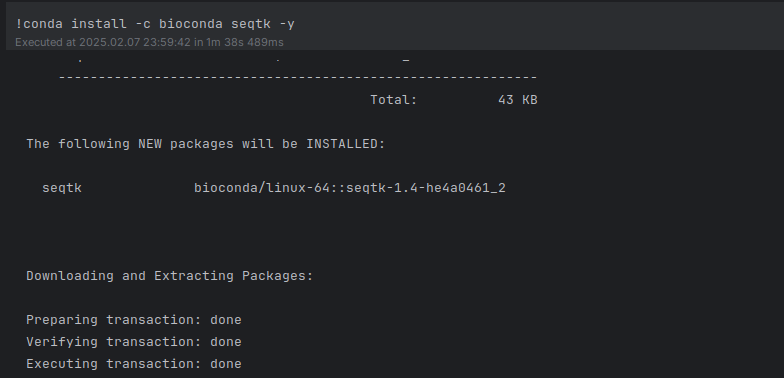
\includegraphics[width=0.8\textwidth]{images/install_cd-hit.png} % Replace with your image file
                \caption{تصب CD-HIT}
                \label{fig:install_cd-hit}
            \end{figure}
            \item اجرای CD-HIT را روی توالی های پروتئین ترجمه شده:\\
            ما توالی‌های پروتئین ترجمه‌شده را با استفاده از CD-HIT با آستانه شباهت 97 درصد خوشه‌بندی کردیم. از دستور زیر استفاده شد:
            \begin{figure}[H]
                \centering
                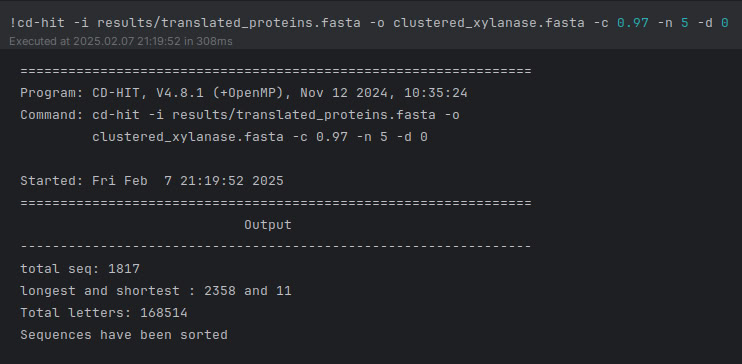
\includegraphics[width=0.8\textwidth]{images/run_cd-hit.jpg} % Replace with your image file
                \caption{اجرای CD-HIT را روی توالی های پروتئین ترجمه شده}
                \label{fig:run_cd-hit}
            \end{figure}
            توضیح پارامترها:
                \begin{itemize}
                    \item \lr{-i} $\leftarrow$ فایل FASTA را وارد کنید (از مرحله 1)
                    \item \lr{-o} $\leftarrow$ فایل خروجی حاوی توالی های خوشه ای
                    \item \lr{-c 0.97} $\leftarrow$ آستانه خوشه بندی (97\% هویت) برای پروتئین ها
                    \item \lr{-n 5} $\leftarrow$ اندازه کلمه برای خوشه بندی (توصیه شده برای پروتئین ها)
                    \item \lr{-d 0} $\leftarrow$ هیچ توضیحات اضافی در خروجی وجود ندارد
                \end{itemize}
                We also clustered nucleotide sequences at a lower similarity threshold (85\%) to account for natural variations in DNA sequences
            \item مشاهده چند خوشه اول
            \begin{figure}[H]
                \centering
                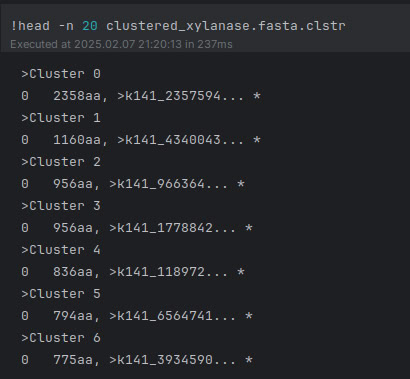
\includegraphics[width=0.5\textwidth]{images/print_top_clusters.jpg} % Replace with your image file
                \caption{مشاهده چند خوشه اول}
                \label{fig:print_top_clusters}
            \end{figure}
        \end{enumerate}
    \subsubsection*{انتخاب توالی های نماینده}
    هنگامی که توالی ها خوشه می شوند، باید یک توالی نماینده برای هر خوشه انتخاب شود. در بیشتر موارد، طولانی ترین دنباله در هر خوشه برای حفظ مرتبط ترین اطلاعات بیولوژیکی انتخاب می شود.
    \begin{figure}[H]
        \centering
        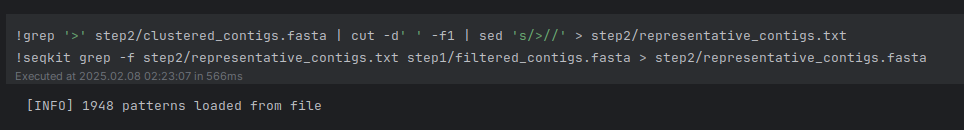
\includegraphics[width=0.8\textwidth]{images/select_representives.png} % Replace with your image file
        \caption{انتخاب توالی های نماینده}
        \label{fig:select_representives}
    \end{figure}
    \subsection*{تفسیر نتایج}

    خوشه‌بندی با موفقیت توالی‌های اضافی را حذف کرد و مجموعه داده‌ها را از 2659 دنباله به 1948 خوشه کاهش داد. بیشتر خوشه ها حاوی تنها 1-5 توالی هستند که نشان دهنده تنوع ژنتیکی بالا در بین ژن های متاژنومی زایلاناز است. نمودار پراکندگی تایید می کند که توزیع طول دنباله تا حد زیادی بدون تغییر باقی می ماند. توالی های نماینده یک مجموعه غیر زائد برای تجزیه و تحلیل بیشتر فراهم می کنند.

    از طریق مرحله 2، ما با موفقیت 2659 توالی زایلاناز متاژنومیک را خوشه بندی کردیم و ضمن حفظ تنوع، افزونگی را کاهش دادیم. توالی های نماینده انتخاب شده از هر خوشه در مرحله 3 برای ویرایش عملکردی بیشتر و تجزیه و تحلیل دامنه حفاظت شده استفاده خواهند شد.


